\section{强子结构和强相互作用}
这一章主要介绍强子（如质子、中子等复合粒子）的内部结构以及它们之间的强相互作用。
首先从强子的对称性性质开始，利用群表示论得到这些对称性的不可约表示，进一步归纳为夸克模型，随后讲解强子的命名规则。
\n{Wolfgang Pauli: Had I foreseen that, I would have gone into botany.}

\subsection{强子的对称性和夸克模型}
\paragraph{夸克模型}随着实验技术的进步，越来越多的粒子被发现，此时粒子的分类成为了一个关键的问题，不可能所有的粒子都是基本粒子。
早期对粒子分类有许多尝试，比如 Fermi 和杨振宁的模型，还有 Sakata 模型等，但都未能成功解释所有粒子。直到最后，Gell-Mann 和 Zweig 根据强子对称性提出了夸克模型，认为强子依旧具有内部结构，是由更基本的夸克组成的，这一理论成功给强子进行了分类。

\begin{figure}[H]
    \centering
    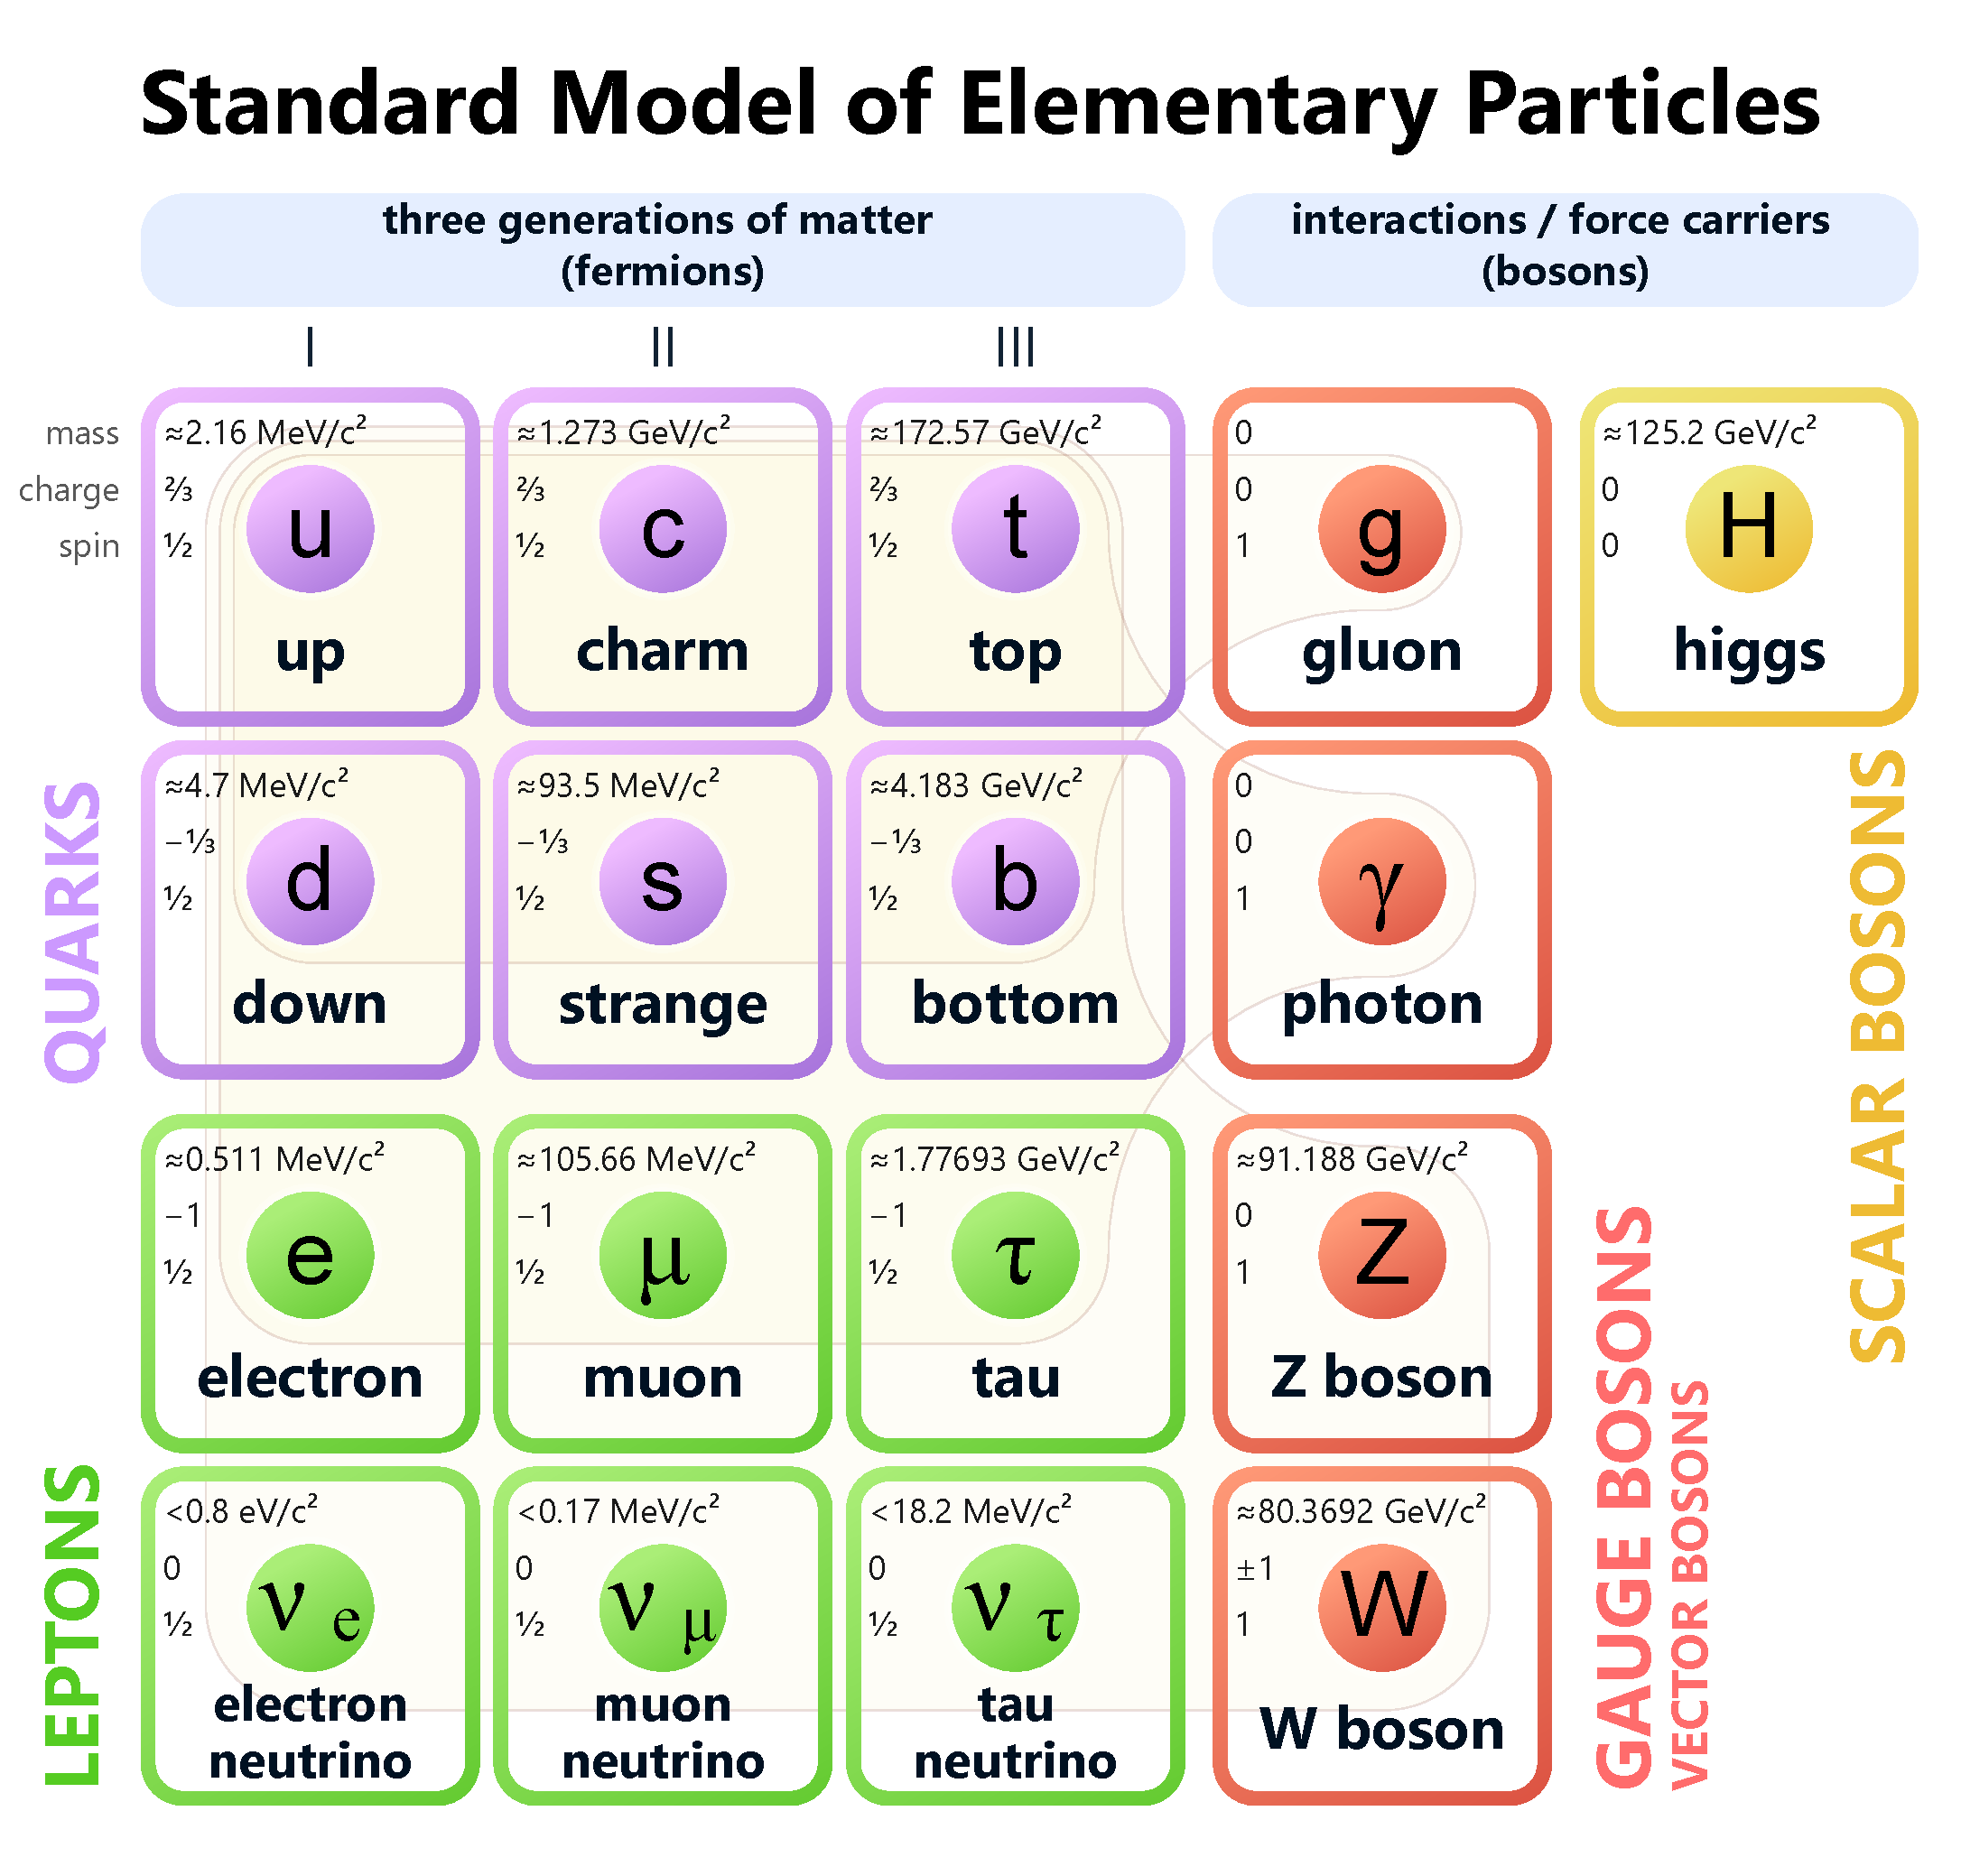
\includegraphics[width=0.6\textwidth]{figs/SM.pdf}
    \caption{粒子物理标准模型}
\end{figure}

在粒子物理标准模型中，夸克是构成物质的最基本单元之一，主要有三类核心特征：
\begin{itemize}
    \item \textbf{自旋统计}：夸克是自旋为 $1/2$ 的费米子，服从费米-狄拉克统计。
    \item \textbf{味道}：根据 GIM 机制，夸克都是成对出现的（一代），目前发现了三代夸克，六个味道，按质量分为：
    \begin{enumerate}
        \item 第一代：上夸克 ($u$)、下夸克 ($d$)；
        \item 第二代：粲夸克 ($c$)、奇异夸克 ($s$)；
        \item 第三代：顶夸克 ($t$)、底夸克 ($b$)。
    \end{enumerate}
    味道主要决定强子的种类和性质。
    \item \textbf{颜色}：颜色自由度的引入是为了服从 Pauli 不相容原理，每种味道的夸克都额外携带一种色荷，通常记为红（R）、绿（G）、蓝（B）。类似电磁相互作用，颜色决定了强相互作用的性质。
\end{itemize}
实验上观测的较多的强子是介子和重子，介子是由一个夸克和一个反夸克组成的束缚态，而重子则是由三个夸克组成的束缚态。

\paragraph{强子对称性及其分类}
\n{虽然 $I_3$ 和 $Q$ 也是可相加性量子数，但是 $I_3$ 已经包含于 $SU(2)_I$ 对称性中了，而 $Q$ 是 $I_3$ 和 $Y$ 的线性组合。}

通过对大量已知强子的性质分析，可以发现强相互作用中存在多种守恒量，这些守恒量对应着内部空间的对称性。主要的对称性包括：
\begin{itemize}
    \item \textbf{同位旋对称性}：对应内部空间的 $SU(2)_I$ 对称性。其守恒量为同位旋 $I$ 及其第三分量 $I_3$。
    \item \textbf{超荷守恒}：对应内部空间的 $U(1)_Y$ 对称性，$Y = b + S + C + B + T$，其中 $b$ 为重子数，$S$ 为奇异数，$C$ 为粲数，$B$ 为底数，$T$ 为顶数。
\end{itemize}

这两种对称性说明，强子是 $I_3$ 和 $Y$ 的共同本征态，并且可以同时测量这两个量。因此，对于强子服从的整体对称性，至少是 $U(1)_Y \otimes SU(2)_I$。如果强子服从其他更高的对称性，那么这个对称性对应的群 $G$ 起码是以 $U(1)_Y \otimes SU(2)_I$ 为子群的。$SU(2)_I$ 是 3 阶 1 秩群而 $U(1)_Y$ 是 1 阶 1 秩群，因此 $G$ 至少是 2 秩群，其中有两个互相对易的生成元对应 $I_3$ 和 $Y$。

另外，强子除了内禀对称性还具有与之正交的空间对称性，具有相同 $I_3$ 和 $Y$ 的强子可以有不同的 $J^{P}$。而满足所有这些性质的，只有 $SU(3)_f$ 群。

\n{这里的 $SU(3)_f$ 指的是 Flavor SU(3)（味道对称性）。这种对称性来源于夸克质量的近似（而不是相同），这个对称性是一个“破缺的对称性”。它在处理 $u, d, s$ 组成的轻强子时非常有效，但对于重夸克系统并不好用。}

$SU(3)_f$ 是三维复空间的幺正幺模矩阵群。它拥有 8 个生成元 $T_i$，通常表示为 $T_i = \frac{1}{2}\lambda_i$。这里的 $\lambda_i$ 被称为 Gell-Mann 矩阵。在这八个生成元中，只有 $\lambda_3$ 和 $\lambda_8$ 是对角矩阵相互对易：
\begin{align}
    [\lambda_3, \lambda_8] = 0
\end{align}
它们构成了该群的最大对易子集，它们分别对应强子的两个可观测量：
\begin{equation}
    I_3 = \frac{1}{2}\lambda_3, \quad Y = \frac{1}{\sqrt{3}}\lambda_8
\end{equation}

$SU(3)_f$ 的基础表示是一个三维矢量空间，其基矢即为三种味道的轻夸克：上夸克 ($u$)、下夸克 ($d$) 和奇异夸克 ($s$)。
夸克的电荷满足广义的盖尔曼-西岛公式：
$$Q = I_3 + \frac{Y}{2} = I_3 + \frac{b + S + C + B + T}{2}$$
由此制约了可观测量算符和 $SU(3)_f$ 群生成元的关系，由此可得夸克具有分数电荷。下表总结了所有夸克及其量子数性质：
\n{因为没系统学过Lie群的表示论，所以这里关于$SU(3)$群的大多地方没有写证明，包括权图的叠加，有空的话可以专门补一补。}
\begin{table}[H]
    \centering
    \renewcommand{\arraystretch}{1.3}
    \setlength{\tabcolsep}{4pt}
    \begin{tabular}{|c|c|c|c|c|c|c|c|c|c|}
    \hline
    \textbf{夸克味道} & \textbf{同位旋} & \textbf{同位旋} & \textbf{奇异数} & \textbf{粲数} & \textbf{底数} & \textbf{顶数} & \textbf{电荷} & \textbf{重子数} & \textbf{组分质量} \\
     & ($I$) & ($I_3$) & ($S$) & ($C$) & ($B$) & ($T$) & ($Q$) & ($b$) & (MeV/$c^2$) \\ \hline
    $u$ & $1/2$ & $1/2$ & $0$ & $0$ & $0$ & $0$ & $2/3$ & $1/3$ & $\sim 310$ \\ \hline
    $d$ & $1/2$ & $-1/2$ & $0$ & $0$ & $0$ & $0$ & $-1/3$ & $1/3$ & $\sim 310$ \\ \hline
    $s$ & $0$ & $0$ & $-1$ & $0$ & $0$ & $0$ & $-1/3$ & $1/3$ & $\sim 500$ \\ \hline
    $c$ & $0$ & $0$ & $0$ & $1$ & $0$ & $0$ & $2/3$ & $1/3$ & $\sim 1600$ \\ \hline
    $b$ & $0$ & $0$ & $0$ & $0$ & $-1$ & $0$ & $-1/3$ & $1/3$ & $\sim 4600$ \\ \hline
    $t$ & $0$ & $0$ & $0$ & $0$ & $0$ & $1$ & $2/3$ & $1/3$ & $\sim 175000$ \\ \hline
    \end{tabular}
    \caption{夸克的量子数与质量表}
\end{table}

利用 $I_3$ 作为横轴，$Y$ 作为纵轴，我们可以将上述粒子绘制在二维平面上，这种几何图形称为权图。

\subsection{介子与重子的构造}
\n{对八重态中的每一个态做SU(3)变换，所得的态仍然在八重态中，单态亦然。}
在夸克模型中，强子是夸克的组合，利用权图的叠加，直观的得到夸克组成的强子。具体操作是：将一个表示（例如反夸克表示）的权图中心，依次平移并重叠在另一个表示（例如夸克表示）的每一个顶点上，所得所有点的集合构成复合体系可能存在的所有状态。
\paragraph{介子的构造}
\n{对介子做 $SU(3)$ 变换，比如 $u \to d$ 且 $\bar{u} \to \bar{d}$，正反夸克要同时变。因为介子态是夸克和反夸克态直积得到的，$g (\ket{q} \otimes \ket{\bar{q}'}) = g\ket{q} \otimes g\ket{\bar{q}'}$。}
介子由一个夸克和一个反夸克组成，其对应的群论分解为 $\mathbf{3} \otimes \mathbf{3^*} = \mathbf{8} \oplus \mathbf{1}$，用夸克和反夸克组合的九种（$3\times 3$）可能的态可以被分解为互不干扰的单态和八重态。
\begin{figure}[H]
    \centering
    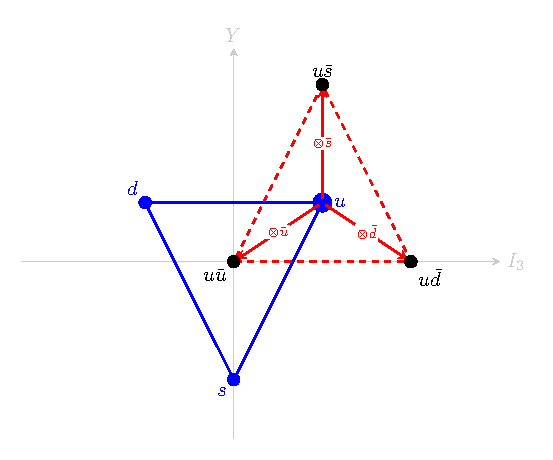
\includegraphics[width=0.6\textwidth]{figs/WeiGAdd.pdf}
    \caption{介子权图的构造}
\end{figure}
按照权图叠加规则，我们先画出由 $u, d, s$ 组成的正三角形，随后以这三个顶点为中心，分别平移并叠加反夸克的倒三角形权图，叠加后的几何结构呈现为一个六边形。


在六边形的外围共有六个顶点，每个顶点对应一个唯一的夸克-反夸克组合，它们具有确定的同位旋和超荷：如顶端的 $u\bar{s}, d\bar{s}$（超荷 $Y=1$），底端的 $s\bar{u}, s\bar{d}$（$Y=-1$），以及水平两侧的 $u\bar{d}, d\bar{u}$（$Y=0$）。而在六边形的几何中心（即原点 $I_3=0, Y=0$ 处），三个反夸克三角形的顶点恰好在此重合，代表了量子数相同的 $u\bar{u}, d\bar{d}$ 和 $s\bar{s}$ 三个态。
\begin{figure}[H]
    \centering
    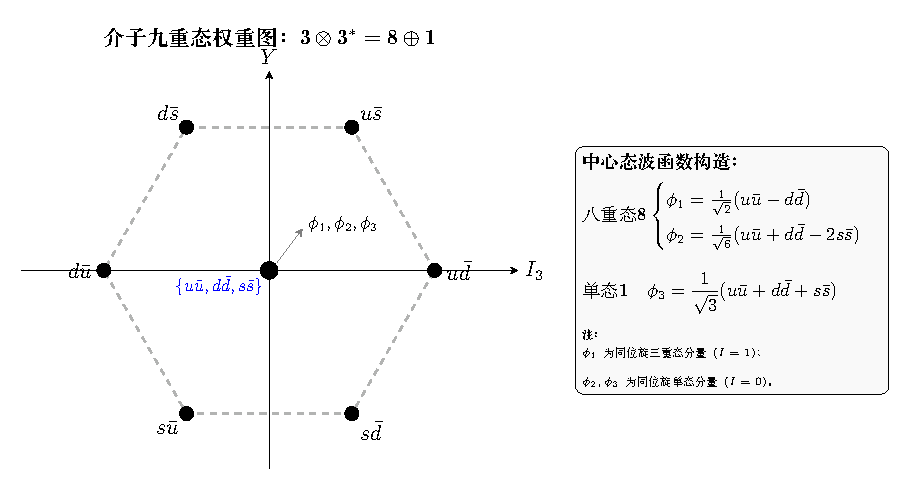
\includegraphics[width=\textwidth]{figs/MwsonWeiG.pdf}
    \caption{介子九重态}
\end{figure}
中间的态具有三个自由度，首先分解出具备全对称性的味单态（在$SU(3)$变换下不变）：

\begin{equation}
    \phi_1 = \frac{1}{\sqrt{3}}(u\bar{u} + d\bar{d} + s\bar{s})
\end{equation}
剩下的两个线性组合则归入味八重态。实验上观测到同位旋 $SU(2)$ 对称性，可以以此构造出同位旋三重态（$I=1$）中的中性成员：
\begin{equation}
    \phi_3 = \frac{1}{\sqrt{2}}(u\bar{u} - d\bar{d})
\end{equation}
以及与上述两者均正交的同位旋单态（$I=0$）成员：
\begin{equation}
    \phi_8 = \frac{1}{\sqrt{6}}(u\bar{u} + d\bar{d} - 2s\bar{s})
\end{equation}
这八个态（六个外围态加上 $\phi_3, \phi_8$）共同构成了味八重态。在相同的味组成下，根据空间对称性的不同，可以形成不同的物理多重态。在实际物理观测中，中心处的味单态 $\phi_1$ 和八重态成员 $\phi_8$ 往往会发生混合，这种味混合现象解释了 $\eta$ 与 $\eta'$ 介子以及 $\omega$ 与 $\phi$ 介子的质量与衰变性质。
\begin{figure}
    \centering
    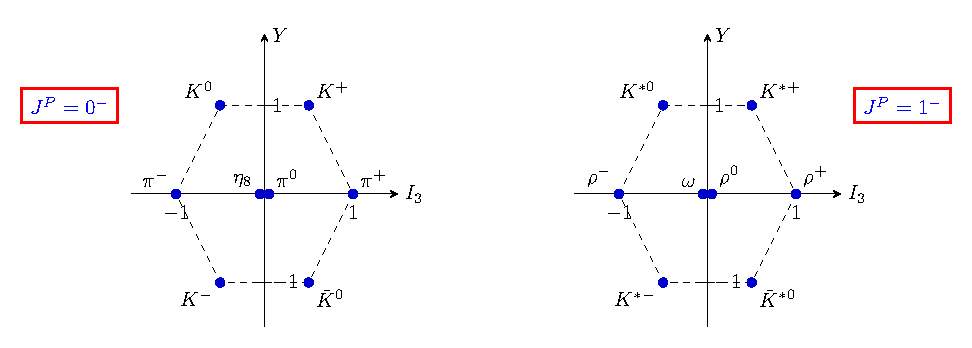
\includegraphics[width=0.8\textwidth]{figs/Meson-space.pdf}
    \caption{不同空间对称性下的介子多重态}
\end{figure}

\paragraph{重子的构造}
重子由三个夸克组成，其对应的群论分解为 $\mathbf{3} \otimes \mathbf{3} \otimes \mathbf{3} = \mathbf{10} \oplus \mathbf{8} \oplus \mathbf{8} \oplus \mathbf{1}$，即由 $3 \times 3 \times 3 = 27$ 种可能的夸克组合态可以分解为一个十重态、两个八重态和一个单态。
对权图中的 27 个态按照交换对称性进行拆分，包含以下四个部分：

\begin{itemize}
    \item \textbf{完全对称（10）}：包含 10 个态，构成重子十重态。这类波函数在交换任意两个夸克的位置时保持不变。
    比如 $\Delta^+$ 粒子的味道波函数为：
    $$\psi_S(\Delta^+) = \frac{1}{\sqrt{3}} \big( |uud\rangle + |udu\rangle + |duu\rangle \big)$$
    当我们交换第一个位置和第二个位置的夸克时，第一项 $|uud\rangle$ 保持不变，第二项 $|udu\rangle$ 与第三项 $|duu\rangle$ 互换，叠加后的总波函数依然是 $\frac{1}{\sqrt{3}} \big( |uud\rangle + |duu\rangle + |udu\rangle \big)$，与原波函数相比完全不变。

    \item \textbf{混合对称（16 = 8 + 8）}：包含 16 个态，分为两个八重态。这些态在交换特定位置的夸克时表现出对称或反对称性质，通常对应自旋 $J=1/2$ 的基态重子。
    \begin{itemize}
        \item \textbf{混合反对称（8）}：波函数对前两个位置（1,2）的交换是反对称的。
        以质子的一个味道波函数分量为例：
        $$\psi_{MA} = \frac{1}{\sqrt{2}} \big( |udu\rangle - |duu\rangle \big)$$
        当我们交换第一个位置和第二个位置的夸克时，波函数变为 $\frac{1}{\sqrt{2}} \big( |duu\rangle - |udu\rangle \big)$，即原波函数符号改变。
        \item \textbf{混合对称（8）}：波函数对前两个位置（1,2）的交换是对称的。
        以质子的另一个味道波函数分量为例：
        $$\psi_{MS} = \frac{1}{\sqrt{6}} \big( |udu\rangle + |duu\rangle - 2|uud\rangle \big)$$
        当我们交换第一个位置和第二个位置的夸克时，前两项 $|udu\rangle$ 和 $|duu\rangle$ 互换，第三项 $-2|uud\rangle$ 保持不变，总波函数与原波函数相比保持不变。
    \end{itemize}

    \item \textbf{完全反对称（1）}：包含 1 个态，构成重子单态。波函数在交换任意两个夸克的位置时符号都会改变。
    该态由 $u, d, s$ 三种味道组成，可以表示为以下 Slater 行列式形式：
    $$\psi_A = \frac{1}{\sqrt{6}} \det \begin{pmatrix} u(1) & d(1) & s(1) \\ u(2) & d(2) & s(2) \\ u(3) & d(3) & s(3) \end{pmatrix}$$
    其中行代表夸克所在的位置（1, 2, 3），列代表夸克的种类。根据行列式的代数性质，交换任意两行（即交换任意两个位置的夸克）会导致整个行列式的值反号。在实际物理中，仅靠味道、自旋和空间部分无法让所有的重子都满足波函数的反对称性，因此必须引入颜色自由度来提供额外的全反对称性。
\end{itemize}
\n{不同颜色、味道和自旋的夸克都源自同一个 Dirac 场的激发，反对易关系 $\{ \hat{a}^\dagger_{f,c,s}(\vec{r}_1), \hat{a}^\dagger_{f',c',s'}(\vec{r}_2) \} = 0$ 使得不同的味道、颜色、自旋（$\pm 1/2$）或者位置的夸克依旧要服从自旋-统计关系，“全同”指相同的本质物理属性（质量、内禀自旋 $1/2$ 等）}
\begin{derivationnote}[重子波函数的全反对称性和颜色自由度]

与介子不同的是，由于重子是三费米子系统，根据全同粒子统计规律，其整体波函数 $\Psi_{\text{总}}$ 必须对任意两个夸克的交换满足全反对称性。重子的完整波函数可以表示为：

$$\Psi_{\text{总}} = \psi_{\text{空间}} \otimes \chi_{\text{自旋}} \otimes \phi_{\text{味道}} \otimes \zeta_{\text{颜色}}$$

波函数中的几个部分，空间和自旋是早就知道的自由度，味道部分源自$SU_f(3)$味对称性，唯独颜色部分没有说明来源。
\n{作业题，可能考}
实际上，它是为了保持重子系统波函数全反对称性额外引入的自由度
考虑基态重子十重态中的 $\Delta^{++}$ 粒子（$uuu$），其量子数如下：
    \begin{enumerate}
        \item \textbf{空间部分}：基态（$L=0$），空间波函数是完全对称的。
        \item \textbf{自旋部分}：三个费米子要么耦合为混合对称性自旋波函数要么耦合为全对称自旋波函数，但是混合对称性自旋波函数会使得整体波函数不存在全反对称性，只能选择全对称性$J=3/2$（如 $\uparrow\uparrow\uparrow$），自旋波函数完全对称。
        \item \textbf{味道部分}：三个 $u$ 夸克，味道波函数是完全对称的。
    \end{enumerate}
    \n{这个构造也意味着重子是多个颜色夸克的耦合，最后呈现色单态。}
    如果只有这三个自由度，总波函数将是完全对称的，这违反了费米子全反对称的统计规律。因此，必须引入一个新的自由度——\textbf{颜色}，且颜色波函数是反对称的：
    $$\zeta_{\text{颜色}} = \frac{1}{\sqrt{6}} \det \begin{pmatrix} R(1) & G(1) & B(1) \\ R(2) & G(2) & B(2) \\ R(3) & G(3) & B(3) \end{pmatrix}$$
\begin{itemize}
    \item \textbf{重子八重态可以有自旋 3/2 吗？重子十重态可以有自旋 1/2 吗？}
    \begin{itemize}
        \item \textbf{十重态（味道全对称）}：重子十重态味道全对称，空间全对称，颜色全反对称性，因此自旋部分必须也是全对称的（即 $J=3/2$），以确保整体波函数的全反对称性。如果尝试匹配自旋 $1/2$（混合对称），则乘积态将不再是全对称。
        \item \textbf{八重态（味道混合对称）}：重子八重态味道混合对称，空间全对称，颜色全反对称性，因此自旋部分必须是混合对称的（即 $J=1/2$），以确保整体波函数的全反对称性。
    \end{itemize}
    \item \textbf{夸克模型中基态重子单态的缺失：}
    味单态呈现全反对称性，基态时空间波函数全对称，颜色波函数全反对称性，而自旋波函数只能拼凑出混合对称或全对称。因此，无法构造出满足全反对称性的整体波函数。
\end{itemize}
\end{derivationnote}

\subsection{介子和重子的命名规则}
正如 $u, d, s$ 组成的强子可以用味道 $SU(3)_f$ 对称性描述，在考虑 $c, b$ 夸克后，理论上味道对称性可以扩充到 $SU(5)_f$。虽然这 5 味夸克的质量相差好几个数量级，使得该对称性已经很难称为物理对称性，但强子分类依然可以按照 $SU(5)_f$ 不可约表示进行。这意味着同一个味道超多重态的自旋、宇称、C 变换因子相同，即同一个超多重态中的粒子具有相同的 $J^{PC}$。

\paragraph{介子的命名规则}
介子是由正反夸克构成的色单态强子体系。夸克自旋为 $1/2$，因此正反夸克的总自旋 $S$ 只能为 0 或 1。设正反夸克间的轨道角动量为 $L$，
则宇称 $P = (-1)^{L+1}$，电荷共轭宇称 $C = (-1)^{L+S}$，对于普通介子还有 $G$ 宇称 $G = (-1)^I C$。

根据 $L$ 和 $S$ 的耦合，正反夸克系统允许的 $J^{PC}$ 如下表所示：
\n{轨道角动量为零的态能量最低，赝标介子$(0^{-+})$和矢量介子$(1^{--})$是介子的基态。}

\begin{table}[H]
    \centering
    \begin{tabular}{|c|c|c|}
    \hline
    \textbf{$L \setminus S$} & \textbf{0} & \textbf{1} \\ \hline
    0 & $0^{-+}$ & $1^{--}$ \\ \hline
    1 & $1^{+-}$ & $0^{++}, 1^{++}, 2^{++}$ \\ \hline
    2 & $2^{-+}$ & $1^{--}, 2^{--}, 3^{--}$ \\ \hline
    3 & $3^{+-}$ & $2^{++}, 3^{++}, 4^{++}$ \\ \hline
    \end{tabular}
    \caption{正反夸克系统可能的 $J^{PC}$}
\end{table}

对于普通介子（$S=C=B=0$），其命名规则依据 $J^{PC}$ 和同位旋 $I$ 划分如下：
\begin{table}[H]
    \centering
    \small
    \renewcommand{\arraystretch}{1.5}
    \begin{tabular}{|c|c|c|c|c|}
    \hline
    \textbf{$J^{PC}$} & \textbf{$(0,2,4\dots)^{-+}$} & \textbf{$(1,2,3\dots)^{--}$} & \textbf{$(0,1,2\dots)^{++}$} & \textbf{$(1,3,5\dots)^{+-}$} \\ \hline
    \textbf{$^{2S+1}L_J$} & $^1(S,D\dots)_J$ & $^3(S,D\dots)_J$ & $^3(P,F\dots)_J$ & $^1(P,F\dots)_J$ \\ \hline
    \textbf{$I=1$} & $\pi$ & $\rho$ & $a$ & $b$ \\ \hline
    \textbf{$I=0$} ($u,d,s$) & $\eta, \eta'$ & $\omega, \phi$ & $f, f'$ & $h, h'$ \\ \hline
    \textbf{$c\bar{c}$ ($I=0$)} & $\eta_c$ & $\psi$ & $\chi_c$ & $h_c$ \\ \hline
    \textbf{$b\bar{b}$ ($I=0$)} & $\eta_b$ & $\Upsilon$ & $\chi_b$ & $h_b$ \\ \hline
    \end{tabular}
    \caption{普通介子分类命名表}
\end{table}

\paragraph{带味介子（$S, C, B \neq 0$）的命名}
对于含有重夸克（$s, c, b$）的介子，其命名不仅是为了分类，更是直接对应其内部夸克组分。核心规则是：\textbf{介子的味道数符号（$S, C, B$）与介子的电荷符号相同}。

我们可以将一个介子符号（例如 $K^{*+}$）拆解为三个部分来解读：

\begin{itemize}
    \item \textbf{1. 主符号（确定重味夸克种类）：}
    \begin{itemize}
        \item $K \Rightarrow$ 奇异介子，含有奇异 ($s$) 或反奇异 ($\bar{s}$) 夸克。
        \item $D \Rightarrow$ 粲介子，含有粲 ($c$) 或反粲 ($\bar{c}$) 夸克。
        \item $B \Rightarrow$ 底介子，含有底 ($b$) 或反底 ($\bar{b}$) 夸克。
    \end{itemize}
    
    \item \textbf{2. 右上角标“*”（确定自旋态）：}
    \begin{itemize}
        \item \textbf{带“*”号}：表示该介子处于\textbf{自旋 $J=1$ 的矢量态}（即正反夸克自旋平行，${}^3S_1$ 态）。
        \item \textbf{无“*”号}：表示该介子处于\textbf{自旋 $J=0$ 的假标量基态}（即正反夸克自旋反平行，${}^1S_0$ 态）。
    \end{itemize}

    \item \textbf{3. 电荷符号（确定正反夸克）：}
    利用“味道数符号 = 电荷符号”规则来判断含有的是“正夸克”还是“反夸克”。
    \begin{itemize}
        \item $Q > 0 \Rightarrow$ 味道数 ($S, C, B$) 为正。
        \item $Q < 0 \Rightarrow$ 味道数 ($S, C, B$) 为负。
    \end{itemize}
\end{itemize}

下表总结了各带味介子的分类与组分判据：
\begin{table}[H]
    \centering
    \renewcommand{\arraystretch}{1.3}
    \small
    \begin{tabular}{|c|c|c|c|c|}
    \hline
    \textbf{分类} & \textbf{判据规则} & \textbf{基态 ($J=0$)} & \textbf{激发态 ($J=1$)} & \textbf{重夸克组分} \\ \hline
    \multirow{2}{*}{\textbf{奇异 ($K$)}} & $S$ 与 $Q$ 同号 ($+$) & $K^+, K^0$ & $K^{*+}, K^{*0}$ & 含 $\mathbf{\bar{s}}$ ($S=+1$) \\ \cline{2-5}
                                       & $S$ 与 $Q$ 同号 ($-$) & $K^-, \bar{K}^0$ & $K^{*-}, \bar{K}^{*0}$ & 含 $\mathbf{s}$ ($S=-1$) \\ \hline
    \multirow{2}{*}{\textbf{粲 ($D$)}} & $C$ 与 $Q$ 同号 ($+$) & $D^+, D^0$ & $D^{*+}, D^{*0}$ & 含 $\mathbf{c}$ ($C=+1$) \\ \cline{2-5}
                                      & $C$ 与 $Q$ 同号 ($-$) & $D^-, \bar{D}^0$ & $D^{*-}, \bar{D}^{*0}$ & 含 $\mathbf{\bar{c}}$ ($C=-1$) \\ \hline
    \multirow{2}{*}{\textbf{底 ($B$)}} & $B$ 与 $Q$ 同号 ($+$) & $B^+, B^0$ & $B^{*+}, B^{*0}$ & 含 $\mathbf{\bar{b}}$ ($B=+1$) \\ \cline{2-5}
                                      & $B$ 与 $Q$ 同号 ($-$) & $B^-, \bar{B}^0$ & $B^{*-}, \bar{B}^{*0}$ & 含 $\mathbf{b}$ ($B=-1$) \\ \hline
    \end{tabular}
    \caption{带味介子命名与组分对照表}
\end{table}

\begin{example}[通过名字推导 $K^{*+}$ 的组分]
    以 $K^{*+}$ 为例，推导过程如下：
\begin{enumerate}
    \item \textbf{看主符号 $K$}：说明它是奇异介子，含有一个 $s$ 或 $\bar{s}$。
    \item \textbf{看右上角 $*$}：说明它是矢量介子（$J=1$），正反夸克自旋平行。
    \item \textbf{看电荷 $+$}：电荷 $Q=+1$。
    \item \textbf{应用规则}：味道数符号与电荷相同 $\Rightarrow$ $S = +1$。
    \item \textbf{定夸克}：
    \begin{itemize}
        \item 奇异夸克 $s$ 的 $S=-1$，反奇异夸克 $\bar{s}$ 的 $S=+1$。因此该粒子含有 \textbf{$\bar{s}$}。
        \item $\bar{s}$ 的电荷为 $+1/3$。
        \item 总电荷需为 $+1$，故另一个轻夸克电荷应为 $+2/3$。查表可知为 $u$ 夸克。
    \end{itemize}
    \item \textbf{结论}：$K^{*+}$ 是由 \textbf{$u\bar{s}$} 组成的自旋为 1 的介子。
\end{enumerate}
\end{example}

\paragraph{重子命名规则}
重子的命名规则大致依赖于\textbf{轻夸克数量}）与\textbf{同位旋}（$I$），可以将一个重子符号拆解为三个步骤来解读：

\begin{itemize}
    \item \textbf{1. 主符号（确定轻夸克 $u/d$ 的数量与同位旋）：}
    这是最核心的分类判据，符号直接告诉我们重子里面有几个“普通”轻夸克：
    \begin{itemize}
        \item $\bm{N, \Delta} \implies$ 含有 \textbf{3 个}轻夸克（即不含 $s, c, b$）。
            \begin{itemize}
                \item $N$：自旋 $1/2$，同位旋 $I = 1/2$。
                \item $\Delta$：自旋 $3/2$，同位旋 $I = 3/2$。
            \end{itemize}
        \item $\bm{\Lambda, \Sigma} \implies$ 含有 \textbf{2 个}轻夸克。
            \begin{itemize}
                \item $\Lambda$：同位旋 $I = 0$（味波函数反对称，通常为味单态）。
                \item $\Sigma$：同位旋 $I = 1$（味波函数对称，通常为味三重态）。
            \end{itemize}
        \item $\bm{\Xi} \implies$ 含有 \textbf{1 个}轻夸克，同位旋 $I = 1/2$。
        \item $\bm{\Omega} \implies$ 含有 \textbf{0 个}轻夸克，同位旋 $I = 0$。
    \end{itemize}

    \item \textbf{2. 下标（确定重夸克成分）：}
    重子必须由 3 个夸克组成。除去主符号确定的轻夸克后，剩下的空位由重夸克填充：
    \begin{itemize}
        \item \textbf{有下标 ($c, b$)}：直接填入对应的粲夸克或底夸克。
        \item \textbf{无下标}：默认剩下的空位全部由\textbf{奇异夸克 ($s$)} 填充。
    \end{itemize}

    \item \textbf{3. 电荷符号（确定具体的轻夸克是 $u$ 还是 $d$）：}
    利用电荷守恒，解出未知的轻夸克具体类型。
\end{itemize}

下表总结了重子符号与夸克组分的对应关系：

\begin{table}[H]
    \centering
    \renewcommand{\arraystretch}{1.4}
    \small
    \begin{tabular}{|c|c|c|c|c|}
    \hline
    \textbf{主符号} & \textbf{轻夸克数 ($u/d$)} & \textbf{重/奇异夸克数} & \textbf{同位旋 $I$} & \textbf{典型组分推导 (无下标 $\to$ 含 $s$)} \\ \hline
    $N$ & \textbf{3} & 0 & $1/2$ & $p(uud), n(udd)$ \\ \hline
    $\Delta$ & \textbf{3} & 0 & $3/2$ & $\Delta^{++}(uuu), \Delta^0(udd)$ \\ \hline
    $\Lambda$ & \textbf{2} & 1 & $0$ & $\Lambda^0(uds)$ \\ \hline
    $\Sigma$ & \textbf{2} & 1 & $1$ & $\Sigma^+(uus), \Sigma^0(uds), \Sigma^-(dds)$ \\ \hline
    $\Xi$ & \textbf{1} & 2 & $1/2$ & $\Xi^0(uss), \Xi^-(dss)$ \\ \hline
    $\Omega$ & \textbf{0} & 3 & $0$ & $\Omega^-(sss)$ \\ \hline
    \end{tabular}
    \caption{重子主符号的含义与基础组分}
\end{table}

\begin{example}[实战：通过名字推导 $\Xi_{cc}^{++}$ 的组分]
这是一个双粲重子，推导过程如下：
\begin{enumerate}
    \item \textbf{看主符号 $\Xi$}：说明含有 \textbf{1 个} 轻夸克 ($u$ 或 $d$)。
    \item \textbf{看下标 $cc$}：说明剩下的 2 个位置被 \textbf{2 个粲夸克 ($c, c$)} 占据。
    \item \textbf{看电荷 $++$}：总电荷 $Q=+2$。
    \item \textbf{计算轻夸克}：
    \begin{itemize}
        \item 已知粲夸克 $c$ 的电荷为 $+2/3$。
        \item 两个粲夸克电荷之和：$2/3 + 2/3 = 4/3$。
        \item 设轻夸克电荷为 $q_l$，则根据 $Q_{\text{总}} = \sum Q_q$，有 $4/3 + q_l = +2$（即 $6/3$）。
        \item 解得 $q_l = +2/3$。查夸克表可知，这是 \textbf{$u$ 夸克}。
    \end{itemize}
    \item \textbf{结论}：$\Xi_{cc}^{++}$ 是由 \textbf{$ucc$} 组成的重子。
\end{enumerate}
\end{example}